\documentclass[a4paper,10pt]{article}

% Paquetes requeridos
\usepackage[utf8]{inputenc}
\usepackage[spanish]{babel}
\usepackage{csquotes}
\usepackage{amsmath, amssymb, amsfonts}
\usepackage{graphicx}
\usepackage[style=apa, backend=biber, natbib=true, language=spanish, url=true]{biblatex}
\usepackage{tocloft} % Para personalizar el índice
\usepackage[left=3.5cm,right=2.5cm,top=3.5cm,bottom=3.8cm]{geometry}
\usepackage{setspace} % Espaciado
\usepackage{titlesec} % Para personalizar los títulos
\usepackage{fancyhdr} % Para personalizar encabezados y pies de página
\usepackage{newtxtext}
\usepackage{listings}
\usepackage{xcolor}
\usepackage{caption}
\usepackage{footnote}
\usepackage{ragged2e}

\makesavenoteenv{figure}
% Configuración para las etiquetas de figura
\captionsetup[figure]{labelformat=empty} % Esto elimina el número de figura y el separador

\pagestyle{fancy}
\fancyhf{} % Limpia encabezados y pies de página
\renewcommand{\headrulewidth}{0pt} % Elimina la línea del encabezado

\addbibresource{referencias.bib}
\DeclareLanguageMapping{spanish}{spanish-apa}
% Configuraciones
\setlength{\parskip}{6pt} % Espacio entre párrafos
\setstretch{1.15} % Espacio entre líneas

\renewcommand{\cftsecleader}{\cftdotfill{\cftdotsep}} % Para puntos en el índice

% Estilos para títulos y subtítulos
\titleformat{\section}
{\normalfont\fontsize{12}{15}\bfseries}{\thesection}{1em}{}
\titleformat{\subsection}
{\normalfont\fontsize{10}{13}\bfseries}{\thesubsection}{1em}{}
\titleformat{\subsubsection}
{\normalfont\fontsize{10.5}{13}\bfseries}{\thesubsubsection}{1em}{}

\usepackage[hypertexnames=false, colorlinks=true, 
linkcolor=blue, 
citecolor=blue, 
urlcolor=blue, 
linkbordercolor={1 1 0}, 
citebordercolor={1 1 0}, 
urlbordercolor={1 1 0}, 
filecolor=blue, 
pdfborderstyle={/S/U/W 1}]{hyperref}

% Definición de formato para Solidity
\lstdefinelanguage{Solidity}{
	keywords={public, private, payable, external, address, modifier, require, if, else, while, for, assembly, switch, case, default, let, contract, uint256, uint8, bool, true, false, function, return, constructor, fallback},
	keywordstyle=\color{blue}\bfseries,
	ndkeywords={},
	ndkeywordstyle=\color{darkgray}\ttfamily,
	identifierstyle=\color{black},
	sensitive=false,
	comment=[l]{//},
	morecomment=[s]{/*}{*/},
	commentstyle=\color{purple}\ttfamily,
	stringstyle=\color{red}\ttfamily,
	morestring=[b]',
	morestring=[b]"
}

\lstset{
	language=Solidity,
	extendedchars=true,
	basicstyle=\small\ttfamily,
	showstringspaces=false,
	showspaces=false,
	numbers=left,
	numberstyle=\tiny,
	showtabs=false,
	tabsize=4
}

% Inicio del documento
\begin{document}
	\pagestyle{empty}
	% Carátula
	\begin{titlepage}
		\centering
		\vspace*{1.5cm}
		{\fontsize{14}{17}\bfseries Solidity en el Metaverso: Un Enfoque Hacia los Contratos Inteligentes y la Blockchain\par}
		{\small Borgo, Martín Alejandro; Molina, Leandro Rodrigo\par}
		{\normalsize Universidad Nacional de Entre Ríos\par}
		{\normalsize Facultad de Ciencias de la Administración\par}
		{\normalsize Licenciatura en Sistemas \par}
		{\small \href{mailto:martinborgo8@gmail.com}{martinborgo8@gmail.com}, \href{mailto:LeandroRodrigoMolina@gmail.com}{LeandroRodrigoMolina@gmail.com}\par}
		
		% Resumen y palabras clave
		{\small \justify\textbf{Abstract.} El Metaverso, se presenta como un conjunto de tecnologías que permite la construcción de mundos virtuales. Donde la tecnología blockchain es uno de los pilares fundamentales, ofreciendo un ecosistema descentralizado y seguro, el cual puede ser expandido en funcionalidades mediante los contratos inteligentes. En este contexto Solidity se ha consolidado como el lenguaje de programación predominante en el desarrollo de contratos inteligentes y aplicaciones descentralizadas dentro de las distintas Blockchain. Sin embargo, a pesar de su amplio uso, presenta problemas relacionados con la seguridad y costos de ejecución. La necesidad de abordar estas limitaciones ha propiciado la creación de lenguajes alternativos, que aspiran a solucionar estas dificultades. Debido a la aparición de cada vez más lenguajes orientados a contratos, es necesario tener en cuenta una serie de principios básicos que todo lenguaje creado para este campo debe seguir. Además los desarrolladores a la hora de seleccionar uno de estos lenguajes deben hacerlo en base a criterios sólidos. Es el objetivo de este artículo presentar tanto las características de diseño de los lenguajes, como también los criterios de selección del lenguaje. \par}
		{\small \justify\textbf{Keywords:} Metaverso, Solidity, Contratos inteligentes, Blockchain.\par}
	\end{titlepage}
	
	%Empezamos a escribir
	\section{Introducción al Trabajo Integrador de Contenidos (TIC)}
	El TIC de la cátedra Lenguajes de Programación (LP), tiene como objetivo general relevar información acerca de temas relacionados directa o indirectamente con el contenido de las unidades temáticas del programa de la cátedra; destacándose especialmente que la presentación y defensa del TIC posibilita además la promoción de la materia. Para el logro del mismo, los alumnos deben arribar a conclusiones en base a la temática seleccionada, presentando y exponiendo su trabajo a fin de desarrollar actitudes de autonomía y oralidad; en base a las pautas de elaboración formales que les son requeridas. En el TIC correspondiente al año en curso, se trabajó en la profundización de conceptos acerca del mundo virtual o universo paralelo denominado Metaverso (Metaverse). Se procurará establecer sus orígenes conceptuales, presente y futuro, relaciones con juegos, inteligencia artificial, Internet de las Cosas (IoT), realidad virtual, realidad alternativa y realidad aumentada, dispositivos de acceso, procesos inmersivos y empresas involucradas que están a la vanguardia tecnológica. Asimismo, se intentará establecer cómo estos conceptos se relacionan e integran principalmente con otros, tales como: evolución, principios de diseño, paradigmas y criterios de evaluación de Lenguajes de Programación y por qué los lenguajes C\# y C++, Java, JavaScript, Python, Solidity, Rust, Swift, HTML, CSS, SQL, y TypeScript, entre otros, son los considerados más relevantes para el Metaverso.
	Asimismo, y a modo introductorio, básico y orientativo, se sugirió al alumnado la revisión de los siguientes recursos: 
	\begin{itemize}
		\item \href{https://www.youtube.com/watch?v=x000E3ziMhs}{METAVERSO: EL NUEVO MUNDO VIRTUAL | Qué es y por qué Facebook, Microsoft y otros apuestan por él}
		\item \href{https://www.youtube.com/watch?v=XIJwITC2DeU}{Qué es el metaverso y cuáles son las dudas que genera este mundo 'gemelo' digital | BBC Mundo}
		\item \href{https://www.xataka.com/basics/que-metaverso-que-posibilidades-ofrece-cuando-sera-real}{Qué es el Metaverso, qué posibilidades ofrece y cuándo será real}
		\item \href{https://academy.binance.com/es/articles/top-7-technologies-that-power-the-metaverse}{Las 7 principales tecnologías que impulsan el metaverso}
		\item \href{https://www.zoomtecnologico.com/2021/12/07/metaverso-zuckerberg/}{¿Cómo respondemos los programadores al metaverso?}
		\item \href{https://tecnovr.net/metaverso-top-lenguajes-de-programacion-para-trabajar/}{Metaverso: Top lenguajes de programación para trabajar}
		\item \href{https://metaverso247.com/metaverso/2022/12/14/cual-es-el-lenguaje-de-programacion-del-metaverso-solidity-vs-javascript/}{¿Cuál es el lenguaje de programación del Metaverso? Solidity vs. JavaScript}
		\item \href{https://blog.soyhenry.com/metaverso-y-programacion-que-rol-tendran-los-desarrolladores/}{Metaverso y programación: ¿qué rol tendrán los desarrolladores?}
		\item \href{https://www.icesi.edu.co/blogs/identidadesavatar/files/2009/01/neal_20stephenson_20-_20snow_20crash.pdf}{SNOW CRASH Neal Stephenson}
	\end{itemize}
	\subsection{Introducción al Metaverso}
	El metaverso, conocido también como universo metafísico o espacio virtual, se refiere a un entorno virtual 3D en línea, donde todos los eventos que ocurren en él se producen en tiempo real y tienen un impacto permanente. La palabra 'metaverso' está compuesta por el prefijo 'meta', que viene del griego \( \mu\varepsilon\tau\acute{\alpha} \) y significa 'más allá' o 'después'. En el contexto del metaverso, este prefijo se refiere a la idea de un universo que va más allá de lo físicamente conocido. Por otro lado, el final '-verso' proviene del latín 'universus', que significa 'todo en uno' o 'entero'. Por lo tanto, el metaverso se puede interpretar como 'un universo alternativo' o 'más allá del universo', refiriéndose a un espacio virtual en línea autónomo que existe más allá de nuestro universo físico.
	
	El término metaverso se popularizó por la novela de Neal Stephenson '\textit{Snow Crash}', en esta novela de género ciencia ficción, más específicamente del subgénero Cyberpunk\footnote{El subgénero Cyberpunk se centra en futuros distópicos donde hay tecnología avanzada y todo lo relacionado a la computación está conectado a una sociedad en decadencia. Ejemplos del subgénero Cyberpunk pueden ser: Neuromancer, Akira, Matrix, Cyberpunk 2077, etc.}. Sin embargo, este término no fue usado por primera vez por Neal, William Gibson en 1980 escribió '\textit{Neuromancer}' donde se presentaba un concepto similar.
	La evolución del término metaverso fue cambiando con el transcurso de los años, en sus inicios, el término nació en la literatura Cyberpunk para representar los futuros distópicos en las novelas de ciencia ficción, para luego avanzar con el paso del tiempo a una definición formal, el cual implica el uso de tecnologías en la vida real. Desde 1992 el metaverso se fue desarrollando constantemente podemos dividir su evolución en cuatro etapas:
	\begin{enumerate}
		\item Etapa Embrionaria (1992-2007): Basada en literatura y arte.
		\item Etapa Primaria (2008-2013): Basado en videojuegos.
		\item Etapa de Reflujo (2014-2019): Restringida por muchos problemas abiertos.
		\item Etapa de Desarrollo (2020-actualidad): Integración de diversas tecnologías para lograr aplicaciones en múltiples campos.
	\end{enumerate}
	Podemos ver cada una de estas etapas, a través del número de publicaciones a lo largo de los años, usando bases de datos como Web of Science y Scopus. Pudiendo observar como las publicaciones por año relacionadas con el Metaverso se van incrementando conforme avanza el desarrollo de distintas tecnologías:
	\begin{figure}[h]
		\centering
		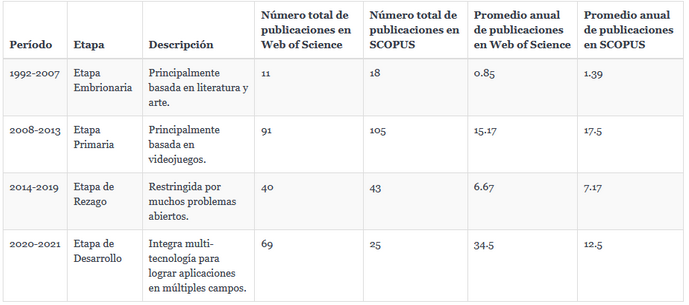
\includegraphics[width=1.0\textwidth]{tablaPublicaciones.PNG}
		\caption{Tabla 1: Cantidad de papers por etapa, traducción propia en a base \textcite{ning2023survey}}
		\label{fig:tabla_publicaciones}
	\end{figure} \\
	Actualmente estamos en la etapa de desarrollo, donde se están integrando y desarrollando diferentes tecnologías para la creación del Metaverso. Estas tecnologías se pueden dividir en cinco aspectos:

	\begin{enumerate}
		\item \textbf{Infraestructura de comunicación y computación:} Se refiere a las bases tecnológicas que hacen posible el Metaverso, principalmente las redes 5G y 6G ofreciendo alta velocidad, baja latencia y conectividad ubicua. Además, el Internet de las Cosas (IoT) es esencial para conectar el Metaverso con el mundo real. La computación en la nube y el Edge Computing son fundamentales para proporcionar la potencia informática necesaria. Lenguajes como \textbf{Python}, \textbf{Go} y \textbf{Elixir} son comúnmente utilizados en la gestión y análisis de redes, la infraestructura de la nube y el análisis de datos en tiempo real.
		\item \textbf{Tecnología de Gestión:} Se centra en cómo se gestionan y mantienen los recursos dentro del Metaverso. Esto incluye la gestión de la energía utilizada por las instalaciones del Metaverso, la asignación y descubrimiento de recursos y la gestión de las interacciones de los usuarios en sesiones. La seguridad y la prevención de ataques también son consideraciones clave en este ámbito, por esa razón lenguajes como \textbf{Rust} y \textbf{C++} son a menudo empleados para la construcción de sistemas de alto rendimiento y de gestión de recursos.
		\item \textbf{Tecnologías fundamentales:} Son las tecnologías esenciales que respaldan las operaciones y el desarrollo del Metaverso. Estas incluyen la realidad virtual y aumentada, la inteligencia artificial, la visión por computadora y la tecnología blockchain. Estas tecnologías permiten la creación de mundos virtuales y la interacción dentro de ellos. Lenguajes como \textbf{Python} para el desarrollo de IA, \textbf{Solidity} para respaldar contratos inteligentes y transacciones seguras, \textbf{C\#} en el desarrollo de RV y RA, gracias a su integración con Unity, son sólo algunos de los muchos existentes.
		\item \textbf{Conexión de Objetos de Realidad Virtual:} Trata sobre cómo los objetos virtuales en el Metaverso interactúan entre sí y con los usuarios. Esto abarca desde la creación de objetos hasta su interacción y eventual destrucción. Lenguajes como \textbf{JavaScript} a través de librerías como \textbf{WebXR API}, \textbf{WebGPU} o \textbf{TreeJS} desempeñan un papel fundamental en la creación de experiencias VR y AR en la web.
		\item \textbf{Convergencia de Realidad Virtual:} Se refiere a la interacción entre el mundo virtual del Metaverso y el mundo real. Esto incluye cómo la información se mueve entre estos dos mundos, cómo los usuarios pueden transitar entre ellos y cómo las acciones en uno pueden influir en el otro. Tecnologías como la AR (Augmented Reality), VR (Virtual Reality), MR (Mixed Reality) utilizan lenguajes como \textbf{Java} o \textbf{C\#} y sus herramientas relacionadas permiten crear aplicaciones AR en dispositivos móviles.
	\end{enumerate}
	Las tecnologías emergentes como la realidad virtual (VR), la realidad aumentada (AR) y las demás tecnologías mencionadas anteriormente están impulsando el desarrollo del metaverso, abriendo nuevas oportunidades en los mercados y el entretenimiento. Tanto así que gigantes corporativos como Meta (anteriormente Facebook) han anunciado sus intenciones de construir un metaverso con fines recreativos y comerciales. Algo muy similar está realizando Microsoft a través de la adquisición de múltiples compañías de videojuegos, y la creación de los HoloLens, un dispositivo de realidad mixta, que permite interactuar con hologramas en el entorno físico. Incluso gigantes de la industria de los videojuegos como Epic Games, con una inversión conjunta de 2.000 millones de dólares de Sony y LEGO, busca construir su visión del metaverso enfocado en la seguridad y diversión de niños y familias. A pesar del impulso, el desarrollo del metaverso enfrenta obstáculos significativos en ámbitos técnicos, éticos y de salud mental, así como en cuestiones de interoperabilidad y compatibilidad. Sin embargo, el camino hacia un metaverso desarrollado en su totalidad enfrenta obstáculos significativos, incluyendo desafíos técnicos, éticos y de salud mental, así como cuestiones de interoperabilidad y compatibilidad. 
	
	Este artículo se centrará en explorar el rol que desempeña la tecnología blockchain, así como sus potenciales aplicaciones en el metaverso mediante el uso de contratos inteligentes. Centrándonos concretamente en el lenguaje de programación Solidity, sus usos, utilidades, ecosistema, limitaciones y sus múltiples herramientas relacionadas\footnote{Para ver una descripción clara de los términos mas comunes del metaverso. véase: \textcite{grandury2022implementacion}}.
	\section{Desarrollo de trabajo}
	En esta sección, se llevará a cabo una revisión bibliográfica que abordará la tecnología Blockchain, los contratos inteligentes y su aplicación en el Metaverso, haciendo énfasis en Solidity, nombrando distintos proyectos que fueron desarrollados usando este lenguaje, el estado actual de su ecosistema y de las herramientas asociadas, resaltando no sólo sus aplicaciones prácticas, sino también las dinámicas y evolución dentro de esta tecnología en expansión. Concluyendo la sección con un análisis del mercado de trabajo de este lenguaje, y presentando una serie de criterios a tener en cuenta a la hora de seleccionar un lenguaje para la construcción de contratos inteligentes.
	
	\subsection{La Blockchain en el Metaverso}
	La tecnología blockchain y sus herramientas afines, como los contratos inteligentes, no solo establecen los cimientos de una economía tangible en el metaverso, sino que también tienen el potencial de mejorar significativamente la seguridad y la integridad de los datos. \textcite{huynh2023blockchain} hablan de como la adquisición de datos en el metaverso es algo fundamental, sobre todo en el entrenamiento de inteligencia artificial y algoritmos de aprendizaje automáticos. Para que todo eso sea posible se requiere información útil y auténtica, en este artículo se discute cómo la tecnología blockchain facilita esta tarea. Ya que, ésta hará que cada uno de los usuarios tengan control sobre su propia información, pudiendo transferir y compartir esta con terceras partes a través de un contrato inteligente. Y por otro lado, debido a que toda esa información se encontrará alojada en la cadena de bloques, nos aseguramos de que esta misma es completamente auténtica y totalmente útil. 
	
	Existen ya una variedad de trabajos que exploran los posibles usos de los contratos inteligentes aplicados sobre todo a la transferencia y protección de datos. \textcite{liu2018enforceable} presentan un marco de trabajo para la transferencia de información y el acceso a datos utilizando contratos inteligentes. A grandes rasgos, los investigadores proponen un proceso en el que las partes acuerdan los términos del contrato por fuera de la cadena de bloques, luego se crea un contrato inteligente personalizado en base a esos términos, proporcionando un acceso único a la parte demandante que le permitirá acceder a los datos guardados en la nube. Si alguna de las partes no cumple con los términos previamente definidos, se recurre a un 'congreso', el cual es un contrato inteligente de votación en el que un jurado decide si hubo un incumplimiento y en caso de que sea necesario se aplica una multa.
	Algo similar es propuesto por \textcite{ouyang2020learning}, el cual presenta un marco de trabajo basado en Federal Learning y contratos inteligentes para entrenar de forma totalmente descentralizada y segura a los algoritmos de inteligencia artificial y aprendizaje automático. Con la diferencia que los autores hablan del concepto de 'Mercados de aprendizaje', donde las distintas partes que entrenan a los modelos de IA pueden comercializar los resultados obtenidos del entrenamiento.
	
	Este tipo de marcos de trabajos representan un gran avance para el metaverso, ya que la inteligencia artificial se presenta como herramienta esencial que potenciará la inmersión de estos mundos virtuales. Desempeñando un papel clave en la personalización de entornos virtuales, la interacción con usuarios y la simulación de mundos virtuales realistas. De ahí que hayan surgido una infinidad de trabajos que exploran los usos de la inteligencia artificial, un ejemplo es el trabajo realizado por (nombre) donde se discute de cómo los NPCs (Non Playable Character) conducidos por inteligencia artificial pueden, mediante el entrenamiento adecuado, adaptarse a cualquier rol que se les quiera asignar. El mismo artículo da el ejemplo como se realizó un experimento donde se entrenó a OpenAI 5 durante 10 meses en Dota 2, logrando ésta derrotar a los campeones mundiales de ese año, demostrando que con el entrenamiento adecuado la inteligencia artificial puede tener el mismo rendimiento que los seres humanos en la realización de tareas difíciles \textcite{yang2022fusing}. Ya dándole un propósito más específico \textcite{hwang2022definition} propone la creación de NPCs impulsados por IA con fines educativos, concretamente los autores mencionan 3 roles que pueden desempeñar estos NPCs, el primer rol es el de profesor, el segundo rol es el de estudiante, que resulta útil para realizar capacitaciones docentes e incluso generar una mayor retroalimentación entre estudiantes. El tercer rol es el de par, el cual está más orientado al apartado de simulación de entornos o recreación de escenarios, siendo extremadamente útil en el área médica y militar, entre muchas otras.
	
	\subsection{Solidity y los Contratos Inteligentes}
	\label{seccion2.2}
	Los contratos inteligentes, no son más que porciones de código escrito en un determinado lenguaje de programación, el cual es almacenado en la blockchain, una vez formando parte de la cadena de bloques estos contratos son inmutables e inmodificables. Ante la necesidad de un lenguaje de programación que esté pensado en su totalidad para la construcción de contratos inteligentes, en 2014 Gavin Wood, cofundador del proyecto Ethereum, propuso la creación de Solidity. En primera instancia este lenguaje fue pensado para ejecutarse en la plataforma de ethereum, pero debido a su popularidad y simplicidad otras plataformas como Cardano o Solana decidieron dar soporte al lenguaje.
	
	Solidity nace como un lenguaje orientado a objetos de tercera generación, el cual cuenta con un fuerte sistema de tipos y una sintaxis sencilla inspirada en lenguajes como C++, Python y JavaScript. Si bien el lenguaje es relativamente nuevo éste se actualiza de manera continua, añadiendo nuevas funcionalidades y corrigiendo errores de forma constante, por estas razones a nivel comercial es ampliamente utilizado para proyectos DeFis (decentralized finance) o DEXs (decentralized exchange) como Aave o SushiSwap, e incluso en la creación de videojuegos play-to-earn como Axie Infinity, Splinterlands o CryptoKitties, entre muchos otros nuevos proyectos que se siguen financiando. En el ámbito académico, también se emplea Solidity para distintos tipos de propósitos como la creación de un sistema de control de inventario entre proveedores y clientes que utiliza contratos inteligentes para realizar los pedidos \parencite{omar2021supply} o un sistema de validación de títulos y certificados académicos \parencite{bousaba2019degree}.
	
	En base a las diferentes aplicaciones brindadas anteriormente podemos notar la amplia adopción que tiene el lenguaje para la construcción de contratos inteligentes. Por esta razón todos los aspectos referidos a la seguridad son cruciales a la hora del desarrollo, ya que cualquier brecha en la seguridad podría derivar en grandes pérdidas económicas o en una filtración masiva de datos sensibles. \textcite{wohrer2018smart}, en su artículo, proponen 6 patrones de diseño enfocados a proveer mayor seguridad y robustez a los contratos inteligentes, a su vez explican criterios generales que todo programador debe tener en cuenta a la hora de escribir código. Otro aspecto importante para tener en cuenta es el consumo de gas\footnote{En cualquier Blockchain la ejecución de un contrato inteligente, así como el almacenamiento de información en esta, cuesta dinero, el gas es una unidad de medición expresada en Gwei utilizado por la red Etherium para designar cuánto cuesta ejecutar una rutina perteneciente a un contrato inteligente. Si bien la cantidad de gas básica necesaria para ejecutar un contrato inteligente depende de la congestión de la red, resulta útil conocerlo ya que mediante este se puede hacer una estipulación de los costos relacionados a cada ejecución.} correspondiente a cada rutina de un contrato, \textcite{marchesi2020design} realiza una recopilación de prácticas y patrones de diseños orientados a la optimización y minimización del consumo de gas. Es importante mencionar que los patrones de diseño no son excluyentes y pueden ser combinados entre sí logrando altos grados de seguridad y reduciendo al máximo el costo de ejecución del contrato.
	
	Este tipo de 'buenas prácticas' combinado con herramientas como GASOL \parencite{albert2020gasol} que calcula la cantidad de gas correspondiente a cada función\footnote{Si bien el compilador de Solidity (solc) puede calcular en tiempo de compilación la cantidad de gas necesaria para ejecutar una función en específico, este cálculo está limitado en algunos casos particulares como aquellos procedimientos que cuentan con un bucle o aquellas que esperan un parámetro variable en tamaño, en estos casos el compilador marcará que el consumo de gas es infinito. GASOL puede realizar estimaciones para ese tipo de funciones ya que utiliza otro tipo de mecanismo para el cálculo del gas.}, lo que permitirá a los programadores crear código más eficiente y seguro. Existen, a su vez, una multitud de herramientas que analizan el código en busca de posibles vulnerabilidades, aunque un estudio realizado por \textcite{durieux2020empirical} mostró que de las 9 herramientas analizadas en su artículo, ninguna pudo detectar dos tipos específicos de vulnerabilidades, no solo eso sino que también se producen una gran cantidad de falsos positivos y falsos negativos, si bien el resultado de este estudio no fue muy alentador, algunas de las herramientas analizadas mostraron mejores resultados para la detección de un tipo específico de vulnerabilidad.
	\subsection{Aplicaciones y Necesidades de la Industria}
	Como se expuso en la sección anterior, Solidity se emplea en una amplia gama de proyectos. No obstante, el mercado laboral asociado tanto a este lenguaje de programación como al sector en el que se emplea, es reducido en comparación con las demás áreas de la industria. Sin embargo, es importante destacar que el sector ha experimentado cambios sustanciales en los últimos años. Según un informe elaborado por Alchemy\footnote{\href{https://www.alchemy.com/blog/web3-developer-report-q2-2023}{Web3 Development Report (Q2 2023)}}, las descargas e instalaciones de los diferentes kits de desarrollo y APIs ofrecidos por la compañía experimentaron un aumento del 37\% interanual, mientras que la cantidad de contratos inteligentes desplegados en sus TestNets ha experimentado un crecimiento interanual del 277\% respectivamente.
	
	Consideramos que este crecimiento podría encontrar obstáculos debido a la escasez de alternativas viables en lo que respecta a los lenguajes de programación empleados en este ámbito. Si bien Solidity es la opción preferida y más utilizada, el lenguaje presenta algunas limitaciones, las cuales desarrollaremos con más detalle en la próxima sección, que pueden dificultar el desarrollo. Por esta razón, todos lo programadores o entidades que quieran construir contratos inteligentes deben tener en cuenta los siguientes criterios a la hora de elegir el lenguaje con el que van a llevar a cabo sus proyecto:
	\begin{itemize}
		\item \textbf{Legibilidad}. Un lenguaje legible ayuda a los programadores a entender el código escrito, además que los recursos de comentarios nos permiten documentar correctamente el código lo cual ayuda al realizar las tareas de mantenimiento. Al mismo tiempo que contar con una sintaxis similar a otros lenguajes hará que el proceso de aprendizaje sea más sencillo.
		\item \textbf{Confiabilidad}. La existencia de un buen sistema y chequeo de tipos, permiten que los programadores pueden corregir los errores de forma temprana y rápida, esto sumado a un adecuado mecanismo de manejo de excepciones, y la restricción del uso de punteros permiten realizar un correcto tratamiento de los errores, además de evitar posibles efectos colaterales en nuestros contratos.
		\item \textbf{Costos}. Los costos asociados al despliegue y posterior ejecución de las rutinas pertenecientes a un contrato inteligente es un factor crucial a tener en cuenta. La eficacia con la que el compilador traduce el código fuente a código objeto, además de el nivel de optimización del código objeto, son factores determinantes a tener en cuenta.
	\end{itemize}
	El ascenso de Solidity en la creación de contratos inteligentes y aplicaciones descentralizadas refleja un escenario prometedor, aunque no exento de desafíos. Las cifras vistas son, si bien alentadoras, subrayan una imperiosa necesidad de abordar las limitaciones que presenta el lenguaje y de explorar y fomentar alternativas que enriquezcan y diversifiquen el campo de desarrollo en la blockchain. En un escenario donde esta tecnología sigue ganando terreno, la solidez y versatilidad de los lenguajes de programación utilizados serán cruciales para sostener e impulsar un crecimiento sostenible y robusto en la industria, permitiendo a su vez, que más desarrolladores aporten de manera eficaz y segura al ecosistema descentralizado.
	\section{Resultados obtenidos}
	Se encontró que el ecosistema de Solidity es uno de los más grandes en comparación con otros lenguajes creados para el mismo propósito como Scilla, Vyper, LLL (Lisp Like Language), entre otros. Esto es gracias a que actualmente Solidity cuenta con gran cantidad de librerías y paquetes que facilitan la construcción de contratos inteligentes seguros, o que permiten integrar estos contratos con servicios web u oráculos\footnote{En Blockchain, los oráculos son servicios brindados por terceras partes que se encargan de verificar, autenticar y consultar información que se encuentra fuera de la cadena de bloques, son extremadamente útiles ya que mediante los oráculos los contratos inteligentes pueden acceder a información del mundo real, como es el precio en tiempo real de divisas nacionales u otras criptomonedas.}, algunos son OpenZeppelin, ChainLink, Web3.js o Ethers.js. A su vez, existe una gran variedad de frameworks como Hardhat, Brownie, Truffle o Foundry que te permiten desplegar y testear tus contratos inteligentes de forma sencilla y sin coste alguno. Sin contar con la gran cantidad de herramientas y patrones mencionadas en la sección \ref{seccion2.2}. Si bien Solidity es, probablemente, la mejor opción para la construcción de contratos inteligentes, el lenguaje cuenta con algunos problemas estructurales debido a su diseño. La existencia de loops y llamadas recursivas hace que sea imposible realizar estimaciones del costo de ejecución además de ser susceptibles a gas attacks. Por otro lado, el lenguaje permite escribir código de más bajo nivel propio de la EVM, si bien esto es una ventaja ya que permite realizar optimizaciones en el consumo de gas y otras operaciones como la delegación de rutinas, el programador debe tener gran conocimiento de cada una de estas instrucciones, de lo contrario podría escribir código inseguro. Es por esta razón que surgieron nuevos lenguajes orientados a la construcción de contratos inteligentes que fueron diseñados mucho más pensado en la seguridad como es el caso de Scilla o Vyper, que dentro de sus principales diferencias está el hecho de que no soportan ningún tipo de loop o llamada recursiva, además de eliminar la posibilidad de escribir código de bajo nivel, además de eliminar los modificadores de funciones, entre otras características más de Solidity que pueden generar errores o vulnerabilidades. El problema principal Scilla o LLL es que utilizan un paradigma funcional puro, haciendo que la construcción de contratos inteligentes se torne confusa, debido a que la mayoría de lenguajes creados para este propósito utilizan el paradigma orientado objetos, esto implica cambiar la forma en cómo se piensa la construcción de los contratos inteligentes, lo cual requiere un mayor esfuerzo por parte de los programadores para aprender a usar el lenguaje en su totalidad.
	
	Si bien el paradigma particular por el que se hayan decantado los diseñadores de lenguajes es relevante, a la hora de diseñar un lenguaje de programación orientado a contratos inteligentes se deben respetar una serie de características base que todo lenguaje creado para este propósito debe tener, entre ellos:
	\begin{itemize}
		\item \textbf{Seguridad}. Dado que cualquier error en el código puede acarrear pérdidas significativas, el lenguaje debe evitar proveer herramientas que nos permita escribir código inseguro o erróneo, esto se puede lograr, como ya mencionamos con anterioridad, mediante la eliminación de las rutinas de más bajo nivel o la eliminación de los loops y llamadas recursivas.
		\item \textbf{Robustez}. El lenguaje debe brindarte herramientas para poder manejar adecuadamente los errores producidos durante la ejecución, concretamente los errores aritméticos como los desbordamientos o divisiones por cero.
		\item \textbf{Reutilización y la Extensibilidad}. Características como la herencia, módulos, mecanismos de abstracción de datos y de procesos, la incorporación de unidades genéricas, permiten a los programadores escribir código altamente reusable, al cual se le pueda añadir nuevas funcionalidades de forma rápida y sencilla.
		\item \textbf{Portabilidad}. Posiblemente una de las características más importantes, ya que al asegurar la compatibilidad con las distintas plataformas existentes, permite que este sea ejecutado sobre múltiples redes.
	\end{itemize}
	A pesar de que Solidity predomina en el entorno de desarrollo de contratos inteligentes, gracias a su extenso repertorio de librerías y herramientas, presenta, no obstante, ciertas vulnerabilidades y defectos propios de su arquitectura y funcionalidad. Lenguajes emergentes como Scilla o Vyper se presentan como alternativas más enfocadas a la seguridad aunque carecen de un uso extendido en el sector. Aun así, se hace patente la necesidad de consolidar lenguajes de programación que integren las características antes desarrolladas, formando así un pilar sólido para el metaverso y tecnologías asociadas.
	\section{Conclusiones}
	Solidity ha establecido un sólido precedente en el desarrollo de contratos inteligentes y aplicaciones descentralizadas, fortaleciendo el ecosistema blockchain con una gama de herramientas, librerías y frameworks que facilitan y optimizan este proceso. No obstante, sus inconvenientes, principalmente en aspectos vinculados con la seguridad y costos de ejecución, revelan la imperante necesidad de explorar y adoptar alternativas que remedien estas debilidades. Aunque existen lenguajes que ofrecen mayor robustez y un enfocado en la seguridad, su adopción ha sido limitada, probablemente debido a sus propios limitaciones y diferencias paradigmáticas en comparación con Solidity. Mirando hacia el futuro, la evolución del desarrollo de contratos inteligentes y la programación en la blockchain requerirán un equilibrio entre seguridad, eficiencia, y accesibilidad para mantener y acelerar su crecimiento, a la vez que se fortalece y asegura la infraestructura subyacente del creciente universo de las finanzas descentralizadas y aplicaciones en la blockchain.
	
	En futuras investigaciones, se llevará a cabo una exploración más profunda con el objetivo de desarrollar un modelo sintáctico y semántico sólido. Este modelo se propone como base para la creación de un lenguaje de programación avanzado que ofrezca seguridad, robustez y una alta portabilidad.
	\section{Referencias}
	\nocite{*}
	\printbibliography[heading=none]
\end{document}
